\section{Property Inference Attacke}\label{sec:property_inference}

Bei der sogenannten Property Inference Attacke versucht ein Angreifer, bestimmte Eigenschaften, Attributwerte, über die Daten eines Modells herauszufinden, welche nur indirekt von einem Modell gelernt wurden und auch nicht bewusst veröffentlicht wurden \cite{P-80}.

Ateniese et al. \cite{P-80} zeigten erstmals, wie so ein Angriff bei Machine Learning Modellen, wie einer Support Vektor Maschine, funktionieren kann.
Dabei handelt es sich um einen White-Box Angriff.
Es wird gezeigt, dass es möglich ist, herauszufinden, ob das angegriffene Modell eine bestimmte Eigenschaft der Daten gelernt hat. 
Um dies zu erreichen, konstruiert der Angreifer mehrere Datenmengen, in denen die zu untersuchende Eigenschaft vorhanden ist oder nicht. 
Anschließend werden diese Datenmengen genutzt, um verschiedene Modelle zu trainieren, welche die gleiche Architektur wie das anzugreifende Modell nutzen.
Diese werden auch Shadow Modelle genannt.
Der Schlüssel dieser Methode ist es, nachfolgend einen Meta-Klassifikator mit diesen Modellen zu trainieren.
Bei Meta-Klassifikatoren handelt es sich um Modelle, welche aus anderen Modellen lernen. 
Konkret werden hierbei die Parameter der Shadow Modelle als Input genutzt, um vorherzusagen, ob die Trainingsdaten die zu untersuchende Eigenschaft besitzen. 
Dies ist möglich, da alle Modelle, das angegriffene Modell und die vom Angreifer trainierten Modelle, eine ähnliche oder sogar identische Architektur haben und dadurch auch zum gleichen Format transformiert werden können.
Außerdem weiß der Angreifer, welches Shadow Modell eine Datenmenge mit oder ohne dem untersuchenden Attributwert nutzt.
Ateniese et al. \cite{P-80} konnten mit diesem Angriff zeigen, dass es möglich ist, herauszufinden, ob ein Sprachmodell mit Daten der Eigenschaft \dq Sprecher mit indischem Dialekt \dq trainiert wurde. 

\begin{figure}[!htb]
    \centering
    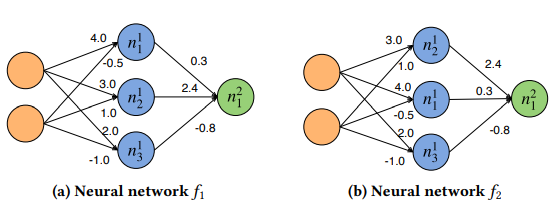
\includegraphics[width=12cm]{figures/permutation_invariance}
    \caption{Permutation eines Neuronalen Netzes \cite{P-11}}
    \label{fig:permutation_invariance}
\end{figure} 

Die Methode von Ateniese et al. \cite{P-80} ist auf diverse Machine Learning Modelle wie Hidden Markov Modelle oder Support Vektor Maschinen ausgelegt, weshalb diese bei Neuronalen Netzen nicht sonderlich gut funktioniert. 
Ganju et al. \cite{P-11} adaptieren den Angriff für Neuronale Netze, indem zwei geeignete Repräsentation für Neuronale Netze genutzt werden, um den Meta-Klassifikator zu trainieren.
Die erste Repräsentation eines Neuronalen Netz basiert auf der Eigenschaft von Neuronalen Netzen, dass die Reihenfolge der Neuronen vertauscht werden kann. 
Abbildung \ref{fig:permutation_invariance} zeigt zwei Neuronale Netze, bei denen die Reihenfolge der Knoten in der ersten Hidden Layer vertauscht ist, jedoch das Modell exakt die gleiche Funktion berechnet.
Diese Eigenschaft kann nun genutzt werden, um die Gewichte jeder Schicht nach der Größe zu sortieren und dadurch eine einheitliche Matrix für verschiedene Permutationen des gleichen Modells zu erhalten.
Die zweite Repräsentation beruht darauf, die Schichten eines Neuronalen Netzes nicht als Vektor, sondern als ein Set darzustellen.
Im Gegensatz zu einem Vektor hat ein Set keine feste Reihenfolge oder Ordnung, sondern ist lediglich eine Menge von Objekten, in diesem Fall eine Menge der Gewichte der Knoten.
Dies sorgt ebenfalls dafür, dass Permutationen des gleichen Modells, in das gleiche Format übertragen werden können.
Ganju et al. \cite{P-11} zeigen anhand des MNIST Datenbestands \cite{D-MNIST}, dass beide Repräsentationsformen die Genauigkeit des Meta-Klassifikators erhöhen können.


Gopinath et al. \cite{P-12} zeigen ein Vorgehen, welches ebenfalls Eigenschaften der Trainingsdaten aus einem Modell extrahiert. 
Dabei handelt es sich eigentlich nicht um einen bösartigen Angriff.
Ziel der Methode ist es, nachvollziehen zu können, warum ein Modell gewisse Entscheidungen trifft, also die Erklärbarkeit eines Modells.
Jedoch ist es nicht auszuschließen, dass die folgende Methode bösartig eingesetzt wird.
Die Methode wird deshalb als White-Box Angriff behandelt, bei welchem die Trainingsdaten ebenfalls bekannt sind.
Gopinath et al. \cite{P-12} zeigen, dass viele Informationen eines Neuronalen Netzes in der Aktivierung der Neuronen steckt, also ob der Output eines Neurons in einem Neuronalen Netz positiv oder negativ ist.
Um die Aktivierung zu messen, wird eine Datenmenge aus den Trainings- und Testdaten gewählt und durch das Modell inferiert.
Anschließend werden die Werte der Neuronen gemessen.
Dabei reicht es, einen Wert in \textbf{on} und \textbf{off} zu unterteilen, wobei \textbf{on} einem Wert größer 0 entspricht und \textbf{off} einem Wert von 0 oder kleiner.
Es ist möglich, ein vergleichbares Vorgehen, bei den Shadow Modellen durchzuführen und die daraus resultierenden Matrizen der Neuronenaktivierug zu nutzen, um einen Meta-Klassifikator zu trainieren.
